% Options for packages loaded elsewhere
\PassOptionsToPackage{unicode}{hyperref}
\PassOptionsToPackage{hyphens}{url}
%
\documentclass[
]{article}
\usepackage{amsmath,amssymb}
\usepackage{lmodern}
\usepackage{ifxetex,ifluatex}
\ifnum 0\ifxetex 1\fi\ifluatex 1\fi=0 % if pdftex
  \usepackage[T1]{fontenc}
  \usepackage[utf8]{inputenc}
  \usepackage{textcomp} % provide euro and other symbols
\else % if luatex or xetex
  \usepackage{unicode-math}
  \defaultfontfeatures{Scale=MatchLowercase}
  \defaultfontfeatures[\rmfamily]{Ligatures=TeX,Scale=1}
\fi
% Use upquote if available, for straight quotes in verbatim environments
\IfFileExists{upquote.sty}{\usepackage{upquote}}{}
\IfFileExists{microtype.sty}{% use microtype if available
  \usepackage[]{microtype}
  \UseMicrotypeSet[protrusion]{basicmath} % disable protrusion for tt fonts
}{}
\makeatletter
\@ifundefined{KOMAClassName}{% if non-KOMA class
  \IfFileExists{parskip.sty}{%
    \usepackage{parskip}
  }{% else
    \setlength{\parindent}{0pt}
    \setlength{\parskip}{6pt plus 2pt minus 1pt}}
}{% if KOMA class
  \KOMAoptions{parskip=half}}
\makeatother
\usepackage{xcolor}
\IfFileExists{xurl.sty}{\usepackage{xurl}}{} % add URL line breaks if available
\IfFileExists{bookmark.sty}{\usepackage{bookmark}}{\usepackage{hyperref}}
\hypersetup{
  hidelinks,
  pdfcreator={LaTeX via pandoc}}
\urlstyle{same} % disable monospaced font for URLs
\usepackage[margin=1in]{geometry}
\usepackage{color}
\usepackage{fancyvrb}
\newcommand{\VerbBar}{|}
\newcommand{\VERB}{\Verb[commandchars=\\\{\}]}
\DefineVerbatimEnvironment{Highlighting}{Verbatim}{commandchars=\\\{\}}
% Add ',fontsize=\small' for more characters per line
\usepackage{framed}
\definecolor{shadecolor}{RGB}{248,248,248}
\newenvironment{Shaded}{\begin{snugshade}}{\end{snugshade}}
\newcommand{\AlertTok}[1]{\textcolor[rgb]{0.94,0.16,0.16}{#1}}
\newcommand{\AnnotationTok}[1]{\textcolor[rgb]{0.56,0.35,0.01}{\textbf{\textit{#1}}}}
\newcommand{\AttributeTok}[1]{\textcolor[rgb]{0.77,0.63,0.00}{#1}}
\newcommand{\BaseNTok}[1]{\textcolor[rgb]{0.00,0.00,0.81}{#1}}
\newcommand{\BuiltInTok}[1]{#1}
\newcommand{\CharTok}[1]{\textcolor[rgb]{0.31,0.60,0.02}{#1}}
\newcommand{\CommentTok}[1]{\textcolor[rgb]{0.56,0.35,0.01}{\textit{#1}}}
\newcommand{\CommentVarTok}[1]{\textcolor[rgb]{0.56,0.35,0.01}{\textbf{\textit{#1}}}}
\newcommand{\ConstantTok}[1]{\textcolor[rgb]{0.00,0.00,0.00}{#1}}
\newcommand{\ControlFlowTok}[1]{\textcolor[rgb]{0.13,0.29,0.53}{\textbf{#1}}}
\newcommand{\DataTypeTok}[1]{\textcolor[rgb]{0.13,0.29,0.53}{#1}}
\newcommand{\DecValTok}[1]{\textcolor[rgb]{0.00,0.00,0.81}{#1}}
\newcommand{\DocumentationTok}[1]{\textcolor[rgb]{0.56,0.35,0.01}{\textbf{\textit{#1}}}}
\newcommand{\ErrorTok}[1]{\textcolor[rgb]{0.64,0.00,0.00}{\textbf{#1}}}
\newcommand{\ExtensionTok}[1]{#1}
\newcommand{\FloatTok}[1]{\textcolor[rgb]{0.00,0.00,0.81}{#1}}
\newcommand{\FunctionTok}[1]{\textcolor[rgb]{0.00,0.00,0.00}{#1}}
\newcommand{\ImportTok}[1]{#1}
\newcommand{\InformationTok}[1]{\textcolor[rgb]{0.56,0.35,0.01}{\textbf{\textit{#1}}}}
\newcommand{\KeywordTok}[1]{\textcolor[rgb]{0.13,0.29,0.53}{\textbf{#1}}}
\newcommand{\NormalTok}[1]{#1}
\newcommand{\OperatorTok}[1]{\textcolor[rgb]{0.81,0.36,0.00}{\textbf{#1}}}
\newcommand{\OtherTok}[1]{\textcolor[rgb]{0.56,0.35,0.01}{#1}}
\newcommand{\PreprocessorTok}[1]{\textcolor[rgb]{0.56,0.35,0.01}{\textit{#1}}}
\newcommand{\RegionMarkerTok}[1]{#1}
\newcommand{\SpecialCharTok}[1]{\textcolor[rgb]{0.00,0.00,0.00}{#1}}
\newcommand{\SpecialStringTok}[1]{\textcolor[rgb]{0.31,0.60,0.02}{#1}}
\newcommand{\StringTok}[1]{\textcolor[rgb]{0.31,0.60,0.02}{#1}}
\newcommand{\VariableTok}[1]{\textcolor[rgb]{0.00,0.00,0.00}{#1}}
\newcommand{\VerbatimStringTok}[1]{\textcolor[rgb]{0.31,0.60,0.02}{#1}}
\newcommand{\WarningTok}[1]{\textcolor[rgb]{0.56,0.35,0.01}{\textbf{\textit{#1}}}}
\usepackage{graphicx}
\makeatletter
\def\maxwidth{\ifdim\Gin@nat@width>\linewidth\linewidth\else\Gin@nat@width\fi}
\def\maxheight{\ifdim\Gin@nat@height>\textheight\textheight\else\Gin@nat@height\fi}
\makeatother
% Scale images if necessary, so that they will not overflow the page
% margins by default, and it is still possible to overwrite the defaults
% using explicit options in \includegraphics[width, height, ...]{}
\setkeys{Gin}{width=\maxwidth,height=\maxheight,keepaspectratio}
% Set default figure placement to htbp
\makeatletter
\def\fps@figure{htbp}
\makeatother
\setlength{\emergencystretch}{3em} % prevent overfull lines
\providecommand{\tightlist}{%
  \setlength{\itemsep}{0pt}\setlength{\parskip}{0pt}}
\setcounter{secnumdepth}{-\maxdimen} % remove section numbering
\ifluatex
  \usepackage{selnolig}  % disable illegal ligatures
\fi

\author{}
\date{\vspace{-2.5em}}

\begin{document}

Análise dos resultados do IDEB da 1° à 5° série da rede pública entre
2005 e 2019 ================

\hypertarget{hipuxf3teses-primuxe1rias}{%
\subsubsection{Hipóteses primárias}\label{hipuxf3teses-primuxe1rias}}

\begin{enumerate}
\def\labelenumi{\arabic{enumi}.}
\tightlist
\item
  O desempenho do sistema educacional dos municípios brasileiros
  evoluiram em taxas de variação semelhantes
\end{enumerate}

\hypertarget{hipuxf3teses-secunduxe1rias}{%
\subsubsection{Hipóteses
secundárias}\label{hipuxf3teses-secunduxe1rias}}

1.1 O desempenho no Sistema de Avaliação da Educação Básica (Saeb) ddos
municípios brasileiros evoluiram em taxas de variação semelhantes

1.2 O fluxo escolar dos municípios brasileiros evoluiram em taxas de
variação semelhantes

\begin{Shaded}
\begin{Highlighting}[]
\FunctionTok{library}\NormalTok{(ggplot2)}
\FunctionTok{library}\NormalTok{(ggridges)}
\FunctionTok{library}\NormalTok{(brazilmaps)}
\FunctionTok{library}\NormalTok{(sf)}
\end{Highlighting}
\end{Shaded}

\begin{verbatim}
## Linking to GEOS 3.9.0, GDAL 3.2.1, PROJ 7.2.1
\end{verbatim}

\begin{Shaded}
\begin{Highlighting}[]
\NormalTok{load\_data\_file }\OtherTok{\textless{}{-}}\NormalTok{ here}\SpecialCharTok{::}\FunctionTok{here}\NormalTok{(}\StringTok{"R"}\NormalTok{, }\StringTok{"load\_data.R"}\NormalTok{)}

\FunctionTok{source}\NormalTok{(load\_data\_file)}
\end{Highlighting}
\end{Shaded}

\begin{verbatim}
## -- Attaching packages --------------------------------------- tidyverse 1.3.1 --

## v tibble  3.1.2          v dplyr   1.0.7     
## v tidyr   1.1.3          v stringr 1.4.0.9000
## v readr   1.4.0          v forcats 0.5.1     
## v purrr   0.3.4

## -- Conflicts ------------------------------------------ tidyverse_conflicts() --
## x dplyr::filter() masks stats::filter()
## x dplyr::lag()    masks stats::lag()

## here() starts at C:/Users/victo/Desktop/PROJ/Current/ideb
\end{verbatim}

\hypertarget{visuxe3o-geral}{%
\subsubsection{Visão geral}\label{visuxe3o-geral}}

\begin{Shaded}
\begin{Highlighting}[]
\NormalTok{df\_ideb\_score }\SpecialCharTok{\%\textgreater{}\%}
  \FunctionTok{filter}\NormalTok{(ideb\_score\_status }\SpecialCharTok{==} \StringTok{"Observado"}\NormalTok{) }\SpecialCharTok{\%\textgreater{}\%}
  \FunctionTok{ggplot}\NormalTok{(}\FunctionTok{aes}\NormalTok{(}\AttributeTok{x =}\NormalTok{ ideb\_score, }
             \AttributeTok{y =}\NormalTok{ ideb\_publication\_year, }
             \AttributeTok{fill =}\NormalTok{ ideb\_publication\_year)) }\SpecialCharTok{+}
  \FunctionTok{geom\_density\_ridges}\NormalTok{(}\AttributeTok{stat =} \StringTok{"binline"}\NormalTok{, }\AttributeTok{alpha =} \FloatTok{0.6}\NormalTok{) }\SpecialCharTok{+}
  \FunctionTok{theme\_minimal}\NormalTok{() }\SpecialCharTok{+}
  \FunctionTok{theme}\NormalTok{(}\AttributeTok{legend.position =} \StringTok{"none"}\NormalTok{)}
\end{Highlighting}
\end{Shaded}

\begin{verbatim}
## `stat_binline()` using `bins = 30`. Pick better value with `binwidth`.

## Warning: Removed 1896 rows containing non-finite values (stat_binline).
\end{verbatim}

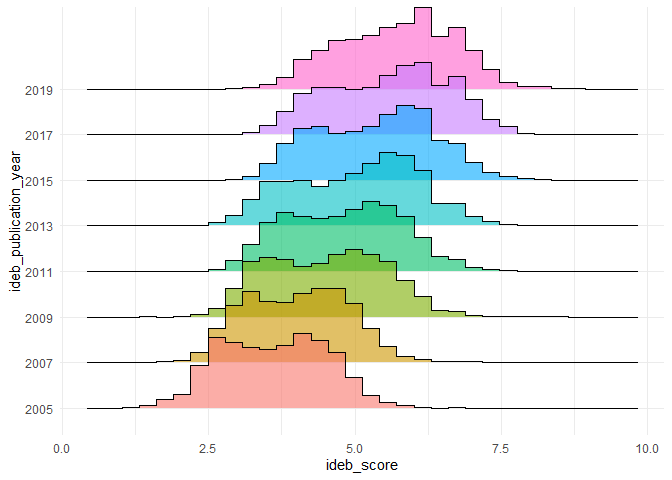
\includegraphics{report_files/figure-gfm/unnamed-chunk-1-1.png}

A partir do histograma acima percebe-ce uma tendência de crescimento do
desempenho escolar no território brasileiro, no entanto esse crescimento
vem acompanhado de maior variação nos dados observados. Outrossim, é
notório a presença de mais de uma moda na distribuição dessa variável
durante todo período de 2005 à 2019, embora neste último ano os valores
tendam para pontuações maiores.

\begin{Shaded}
\begin{Highlighting}[]
\NormalTok{counties\_map }\OtherTok{\textless{}{-}} \FunctionTok{get\_brmap}\NormalTok{(}\StringTok{"City"}\NormalTok{) }
\end{Highlighting}
\end{Shaded}

\begin{Shaded}
\begin{Highlighting}[]
\NormalTok{ideb\_counties\_map }\OtherTok{\textless{}{-}}\NormalTok{ counties\_map }\SpecialCharTok{\%\textgreater{}\%}
  \FunctionTok{mutate}\NormalTok{(}\AttributeTok{City =} \FunctionTok{as.character}\NormalTok{(City)) }\SpecialCharTok{\%\textgreater{}\%}
  \FunctionTok{left\_join}\NormalTok{(df\_ideb\_score,}
            \AttributeTok{by =} \FunctionTok{c}\NormalTok{(}\StringTok{"City"} \OtherTok{=} \StringTok{"county\_id"}\NormalTok{))}
\end{Highlighting}
\end{Shaded}

\begin{Shaded}
\begin{Highlighting}[]
\NormalTok{ideb\_counties\_map }\SpecialCharTok{\%\textgreater{}\%}
  \FunctionTok{filter}\NormalTok{(ideb\_score\_status }\SpecialCharTok{==} \StringTok{"Observado"}\NormalTok{) }\SpecialCharTok{\%\textgreater{}\%}
  \FunctionTok{ggplot}\NormalTok{() }\SpecialCharTok{+}
  \FunctionTok{geom\_sf}\NormalTok{(}\FunctionTok{aes}\NormalTok{(}\AttributeTok{fill =}\NormalTok{ ideb\_score),}
          \AttributeTok{colour =} \StringTok{"transparent"}\NormalTok{, }\AttributeTok{size =} \FloatTok{0.1}\NormalTok{) }\SpecialCharTok{+}
  \FunctionTok{scale\_fill\_continuous}\NormalTok{(}\AttributeTok{type =} \StringTok{"viridis"}\NormalTok{) }\SpecialCharTok{+}
  \FunctionTok{facet\_wrap}\NormalTok{(}\SpecialCharTok{\textasciitilde{}}\NormalTok{ideb\_publication\_year) }\SpecialCharTok{+}
  \FunctionTok{theme}\NormalTok{(}\AttributeTok{panel.grid =} \FunctionTok{element\_line}\NormalTok{(}\AttributeTok{colour =} \StringTok{"transparent"}\NormalTok{),}
        \AttributeTok{panel.background =} \FunctionTok{element\_blank}\NormalTok{(),}
        \AttributeTok{axis.text =} \FunctionTok{element\_blank}\NormalTok{(),}
        \AttributeTok{axis.ticks =} \FunctionTok{element\_blank}\NormalTok{())}
\end{Highlighting}
\end{Shaded}

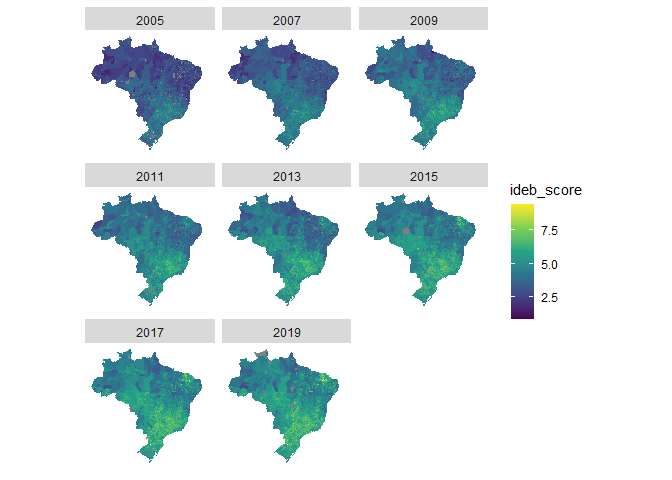
\includegraphics{report_files/figure-gfm/unnamed-chunk-4-1.png}
Segmentando por município e por ano de publicação do IDEB é possível
observar a melhoria do desempenho do sistema educacional nos anos
inicias do enisno fundamental. Em 2005 existia uma predominância
nacional da pontuação entre 2.5 e 5 no IDEB, somente parte dos
territórios da região centro-oeste, sudeste e sul alcançaram indicadores
acima de 5. Nos anos sucessores, ocorre o espalhamento dessa pontuação,
embora ainda restrito às regiões supracitadas.No entanto, em
contrapartida aos seus vizinhos, os municípios Cearences ganham maior
representatividade nessa faixa de desempenho (entre 5 e 7.5), fenômeno
este que se acentua a partir do IDEB de 2011. Para uma visualização
melhor dessa suposta discrepância do desempenho do sistema educacional
nos munícipios brasileiros, é necessário obter uma medida suavizada
baseada nos seus vizinhos. A fim de alcançar esse objetivo utilizou-se a
regra de contiguidade da rainha de primeira ordem.

\begin{Shaded}
\begin{Highlighting}[]
\NormalTok{get\_ideb\_spatial\_lag\_dir }\OtherTok{\textless{}{-}}\NormalTok{ here}\SpecialCharTok{::}\FunctionTok{here}\NormalTok{(}\StringTok{"R"}\NormalTok{, }\StringTok{"get\_ideb\_spatial\_lag.R"}\NormalTok{)}

\FunctionTok{source}\NormalTok{(get\_ideb\_spatial\_lag\_dir)}
\end{Highlighting}
\end{Shaded}

\begin{verbatim}
## Carregando pacotes exigidos: sp

## Carregando pacotes exigidos: spData

## To access larger datasets in this package, install the spDataLarge
## package with: `install.packages('spDataLarge',
## repos='https://nowosad.github.io/drat/', type='source')`

## Warning in lag.listw(ideb_queen_weights, df_ideb$ideb_score, NAOK = TRUE): NAs
## in lagged values

## Warning in lag.listw(ideb_queen_weights, df_ideb$ideb_score, NAOK = TRUE): NAs
## in lagged values

## Warning in lag.listw(ideb_queen_weights, df_ideb$ideb_score, NAOK = TRUE): NAs
## in lagged values

## Warning in lag.listw(ideb_queen_weights, df_ideb$ideb_score, NAOK = TRUE): NAs
## in lagged values

## Warning in lag.listw(ideb_queen_weights, df_ideb$ideb_score, NAOK = TRUE): NAs
## in lagged values

## Warning in lag.listw(ideb_queen_weights, df_ideb$ideb_score, NAOK = TRUE): NAs
## in lagged values

## Warning in lag.listw(ideb_queen_weights, df_ideb$ideb_score, NAOK = TRUE): NAs
## in lagged values

## Warning in lag.listw(ideb_queen_weights, df_ideb$ideb_score, NAOK = TRUE): NAs
## in lagged values
\end{verbatim}

\begin{Shaded}
\begin{Highlighting}[]
\NormalTok{ideb\_counties\_map\_queen\_weights }\SpecialCharTok{\%\textgreater{}\%}
  \FunctionTok{ggplot}\NormalTok{() }\SpecialCharTok{+}
  \FunctionTok{geom\_sf}\NormalTok{(}\FunctionTok{aes}\NormalTok{(}\AttributeTok{geometry =}\NormalTok{ geometry, }\AttributeTok{fill =}\NormalTok{ ideb\_score\_lag),}
          \AttributeTok{colour =} \StringTok{"transparent"}\NormalTok{, }\AttributeTok{size =} \FloatTok{0.1}\NormalTok{) }\SpecialCharTok{+}
  \FunctionTok{scale\_fill\_continuous}\NormalTok{(}\AttributeTok{type =} \StringTok{"viridis"}\NormalTok{) }\SpecialCharTok{+}
  \FunctionTok{facet\_wrap}\NormalTok{(}\SpecialCharTok{\textasciitilde{}}\NormalTok{ideb\_publication\_year) }\SpecialCharTok{+}
  \FunctionTok{theme}\NormalTok{(}\AttributeTok{panel.grid =} \FunctionTok{element\_line}\NormalTok{(}\AttributeTok{colour =} \StringTok{"transparent"}\NormalTok{),}
        \AttributeTok{panel.background =} \FunctionTok{element\_blank}\NormalTok{(),}
        \AttributeTok{axis.text =} \FunctionTok{element\_blank}\NormalTok{(),}
        \AttributeTok{axis.ticks =} \FunctionTok{element\_blank}\NormalTok{())}
\end{Highlighting}
\end{Shaded}

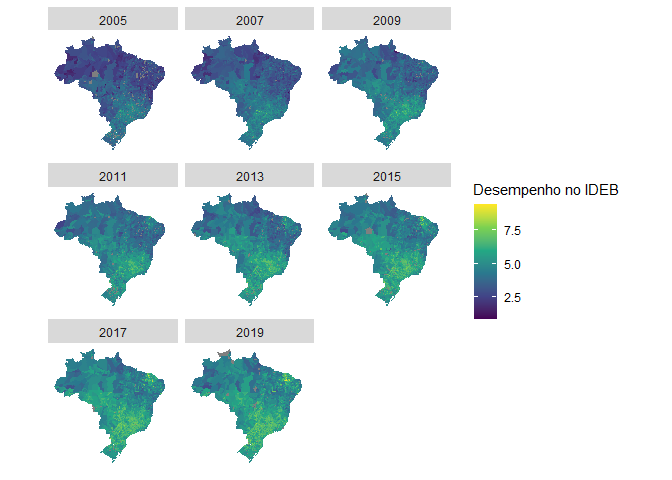
\includegraphics{report_files/figure-gfm/unnamed-chunk-5-1.png}

\hypertarget{referuxeancias}{%
\subsubsection{Referências}\label{referuxeancias}}

\begin{enumerate}
\def\labelenumi{\arabic{enumi}.}
\item
  \url{https://spatialanalysis.github.io/lab_tutorials/Applications_of_Spatial_Weights.html}
\item
  \url{https://mgimond.github.io/Spatial/spatial-autocorrelation-in-r.html}
\end{enumerate}

\end{document}
